\section{Radioaktiv yemirilish qonuni}


\begin{enumerate}

\item Radonning yarim yemirilish davri 90 soatga teng. Boshlang‘ich holatda $2\cdot 10^{21}$ ta atomdan tashkil topgan Radon moddasining 270 soatdan so‘ng nechta atomi qoladi?
\begin{enumerate}[label=\Alph*)]
\item $10^{21}$ ta.
\item $2,5\cdot 10^{21}$ ta.
\item $2,5\cdot 10^{20}$ ta.
\item $2\cdot 10^{20}$ ta.
\end{enumerate}

\item Yarim yemirilish davri 140 sutka bo‘lgan Poloniy izotopining 140 sutkadan keyin qolgan atomlar soni $8\cdot 10^{20}$ ta bo‘lsa, yemirilishdan oldin nechta atomi bo‘lgan?
\begin{enumerate}[label=\Alph*)]
\item $1,2\cdot 10^{21}$ ta.
\item $1,8\cdot 10^{21}$ ta.
\item $1,6\cdot 10^{21}$ ta.
\item $2,4\cdot 10^{21}$ ta.
\end{enumerate}

\item Massasi 3,2 kg bo‘lgan Uran izotopining qancha vaqtdan keyin 0,2 kg massasi yemirilmay qoladi (yil)? Bu izotopning yarim yemirilish davri 250 000 yilga teng.
\begin{enumerate}[label=\Alph*)]
\item $10^6$.
\item $10^5$.
\item $2\cdot 10^6$.
\item $1,5\cdot 10^6$.
\end{enumerate}

\item Biror radioaktiv izotopning yarim yemirilish davri T=5 yil bo‘lib, yadrolarning umumiy soni $N_0=10^{11}$ ta bo‘lsa, t=35 yildan so‘ng bu izotopning nechta (N) radioaktiv yadrosi qoladi?
\begin{enumerate}[label=\Alph*)]
\item $3,1\cdot 10^9$.
\item $7,8\cdot 10^8$.
\item $1,6\cdot 10^9$.
\item $3,9\cdot 10^8$.
\end{enumerate}

\item $4,8\cdot 10^{21}$ ta atomi bo‘lgan Neptuniy izotopining 112 sutkadan keyin qolgan atomlar soni $1,2\cdot 10^{21}$ ta bo‘lsa, yarim yemirilish davrini toping (sutka).
\begin{enumerate}[label=\Alph*)]
\item 72.
\item 10.
\item 56.
\item 38.
\end{enumerate}

\item Elementning yarim yemirilish davri 70 kun. 35 kundan so‘ng radioaktiv yadrolarning necha foizi qoladi?
\begin{enumerate}[label=\Alph*)]
\item 75.
\item 50.
\item 70.
\item 30.
\end{enumerate}

\item Uchta yarim yemirilish davri o‘tgach, radioaktiv atomlarning qanday qismi qoladi (\%)?
\begin{enumerate}[label=\Alph*)]
\item 12,5.
\item 25.
\item 50.
\item 75.
\end{enumerate}

\item Yarim yemirilish davri 6000 yil bo‘lgan radioaktiv moddaning 1000 ta atomi 25 s vaqtda yemirildi. Uning aktivligini toping (Bq).
\begin{enumerate}[label=\Alph*)]
\item 56.
\item 18.
\item 64.
\item 40.
\end{enumerate}

\item Yarim yemirilish davri 2019 yil bo‘lgan radioaktiv moddaning boshlang‘ich aktivligi 50 Bq ga teng bo‘lsa, 1 min ichida nechta atomi yemiriladi?
\begin{enumerate}[label=\Alph*)]
\item 500.
\item 1800.
\item 4000.
\item 3000.
\end{enumerate}

\item Radioaktiv elementning aktivligi 8 sutkada 4 marta kamaydi. Yarim yemirilish davrini toping (sutkalarda).
\begin{enumerate}[label=\Alph*)]
\item 2.
\item 4.
\item 6.
\item 16.
\end{enumerate}

\item Yarim yemirilish davri $T=2$ oy bo‘lgan radioaktiv izotopning boshlang‘ich massasi $m_0=1,6$ g bo‘lsa, $t=300$ kundan keyin uning necha milligrammi yemirilmay qoladi?
\begin{enumerate}[label=\Alph*)]
\item 20.
\item 280.
\item 50.
\item 100.
\end{enumerate}

\item Radioaktiv kumushning aktivligi 810 sutkada 8 marta kamaydi. Uning yarim yemirilish davrini toping (sutkalarda).
\begin{enumerate}[label=\Alph*)]
\item 110.
\item 170.
\item 270.
\item 370.
\end{enumerate}

\item Radiyda $25\cdot 10^6$ ta atom bor. Agar radiyning yarim yemirilish davri 1620 yil bo‘lsa, 1 sutkada qancha atom yemiriladi?
\begin{enumerate}[label=\Alph*)]
\item 2.
\item 29.
\item 47.
\item 93.
\end{enumerate}

\item O‘rtacha yashash vaqti 300 yil bo‘lgan radioaktiv preparatning aktivligi 70 atom/s bo‘lgan vaqtdan boshlab 1 minut ichida nechta atomi yemiriladi?
\begin{enumerate}[label=\Alph*)]
\item 420.
\item 4200.
\item 21000.
\item 350.
\end{enumerate}

\item Rasmda radioaktiv preparat aktivligining vaqtga bog‘lanish grafigi tasvirlangan. 0,05 s da nechta radioaktiv yadro parchalanadi?

\begin{center}
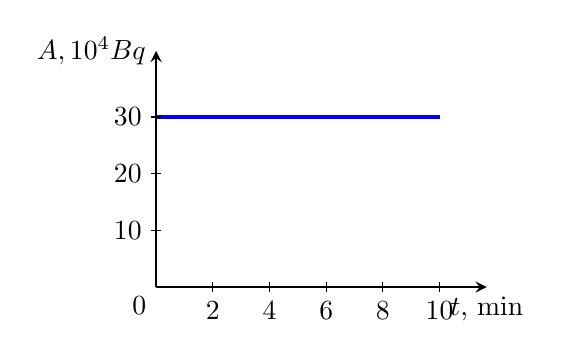
\begin{tikzpicture}[scale=1.2, >=stealth]
  \draw[->, thick] (0,0) -- (3.5,0) node[below] {$t$, min};
  \draw[->, thick] (0,0) -- (0,2.5) node[left] {$A, 10^4\text{ Bq}$};
  \node[below left] at (0,0) {0};
  
  \draw[ultra thick, blue] (0,1.8) -- (3.0,1.8);
  
  \foreach \x/\l in {0.6/2, 1.2/4, 1.8/6, 2.4/8, 3.0/10} {
    \draw (\x,0.05) -- (\x,-0.05) node[below] {\l};
  }
  \foreach \y/\l in {0.6/10, 1.2/20, 1.8/30} {
    \draw (0.05,\y) -- (-0.05,\y) node[left] {\l};
  }
\end{tikzpicture}
\end{center}

\begin{enumerate}[label=\Alph*)]
\item 7,5 ming.
\item 30 ming.
\item 60 ming.
\item 15 ming.
\end{enumerate}

\item Vanadiy--48 izotopining yarim yemirilish davri 16,1 sutka. Shu izotopning o‘rtacha yashash vaqtini (sutka) aniqlang.
\begin{enumerate}[label=\Alph*)]
\item 11,2.
\item 16,1.
\item 23,2.
\item 32,2.
\end{enumerate}

\item To‘g‘ri tasdiqlarni ko‘rsating. Yarim yemirilish davri:
1) radioaktiv jism massasi ortishi bilan ortadi;
2) vaqt o‘tishi bilan kamayadi;
3) jismda sodir bo‘ladigan kimyoviy o‘zgarishlarga bog‘liq emas;
4) jism molekulalarining kimyoviy o‘zgarishiga bog‘liq.
\begin{enumerate}[label=\Alph*)]
\item 1.
\item 2.
\item 3.
\item 4.
\end{enumerate}

\end{enumerate}







\begin{table}[!ht]
\centering
\begin{tabular}{|c|c|c|c|c|c|c|c|c|c|c|}
\hline
1c & 2c & 3a & 4b & 5c & 6c & 7a & 8d & 9d & 10d & 11c \\ \hline
12c & 13b & 14b & 15d & 16c & 17c & & & & & \\ \hline
\end{tabular}
\end{table}